\documentclass{article}
\usepackage{graphicx} % Required for inserting images
\begin{document}
\title{The Impact of Trade Union Dynamics on Income Inequality Trends in European Union Countries}
\author{Jacopo Binati}
\date{Academic Year: 2023 - 2024}
\maketitle
\section{Introduction}

The ever-shifting landscape of the global economy has placed a spotlight on the intricate connection between labour practices and the growing issue of economic inequality (ILO, n.d.). Within the multifaceted mechanisms influencing labour market dynamics, collective bargaining emerges as a crucial tool for shaping fair employment conditions and equitable wage distribution (ILO, n.d.). Collective bargaining, a well-established process of negotiation between employers and organized worker representatives, fosters agreements that regulate working conditions, salaries, benefits, and other aspects of worker compensation and rights. It has been championed as a potential equalizer within the labor market. The theory proposes that by empowering workers to negotiate collectively, they can achieve a more just distribution of income, enhance job security, and improve working conditions. This, in turn, could potentially address some of the root causes of economic inequality (Schmidt and Strauss 1976). However, the effectiveness and impact of collective bargaining are contingent upon various factors including the legal and regulatory framework, the strength and representativeness of labour unions, the economic context, and the adaptability of these institutions to changing labour market conditions. This analysis delves deeper into the complex relationship between collective bargaining and economic inequality. We will explore the theoretical underpinnings of collective bargaining as an equalizer and examine the empirical evidence regarding its effectiveness. We will also consider the various factors that influence the success of collective bargaining efforts and their ultimate impact on reducing economic inequality.

\section{Methodology}

This paper is intended to shed light on the intricate relationship between trade union coverage and inequality, offering a comprehensive exploration beyond mere statistical correlations to understand the underlying mechanisms, societal impacts, and policy implications. The effectiveness and impact of collective bargaining are contingent upon various factors including the legal and regulatory framework, the strength and representativeness of labour unions, the economic context, and the adaptability of these institutions to changing labour market conditions. By examining empirical evidence, case studies, and theoretical frameworks, insight will be provided into the conditions under which collective bargaining most effectively reduces inequality and the challenges and opportunities it presents in the contemporary economic landscape. This project delves into the significant role Trade Unions and Collective Bargaining Coverage have played in addressing Income Inequality across various EU countries over the past two decades. Focusing on Austria, Belgium, Czechia, Denmark, Estonia, Finland, France, Germany, Greece, Hungary, Iceland, Ireland, Italy, Latvia, Lithuania, Luxembourg, Netherlands, Norway, Poland, Portugal, Slovak Republic, Slovenia, Spain, Sweden, Switzerland, and the United Kingdom, it aims to closely examine the relationship between two key variables: the Coverage and Density of labour unions. Collective Bargaining Coverage, as defined by the ILO, refers to the extent to which workers' wages and employment conditions are governed by collective agreements. Meanwhile, Trade Union Density measures the proportion of employees affiliated with a union relative to the total workforce, with net density considering only those actively employed.  

\newpage

\section{A Nuanced Exploration: Trade Union Coverage and Income Inequality}

The intricate relationship between trade union coverage and income inequality demands a nuanced exploration that transcends mere statistical correlations. This study delves deeper, aiming to illuminate the underlying mechanisms, societal impacts, and policy implications of this dynamic. Recognizing the contingent nature of collective bargaining effectiveness, we acknowledge several factors influencing its success: the legal and regulatory framework, union strength and representativeness, economic context, and adaptability to the evolving labor market's challenges, such as the rise of the gig economy and automation. Drawing inspiration from the work of Card (1996) and Goesling (2009), this research employs a multi-faceted approach. We leverage empirical evidence from reputable sources like Eurostat and OECD databases, focusing on data related to trade union coverage (encompassing both density and coverage rate), income inequality metrics (like the Gini coefficient), and relevant control variables for EU countries over the past two decades. This timeframe allows us to capture the potential impact of recent economic shifts, reforms, and the eastward expansion of the EU. Complementing this quantitative analysis, in-depth case studies will be conducted for a selection of EU countries exhibiting diverse levels of trade union coverage and density. These qualitative investigations will explore the specific mechanisms through which trade union activity shapes wage inequality within each chosen nation. The selection criteria for case studies will focus on EU countries exhibiting diverse characteristics across four key dimensions. First, we will examine the legal frameworks of each country, assessing whether legal structures support and protect collective bargaining rights or conversely restrict union activity. Second, the strength and representativeness of unions will be evaluated. This includes analyzing how well-organized unions are and how effectively they represent the interests of a broad range of workers, particularly those in precarious or non-standard employment arrangements. Third, the economic structure of each chosen country

\section{Model building}

This analysis is rooted in datasets obtained from the Organisation for Economic Cooperation and Development (OECD) statistics and World Bank Data, targeting an array of variables pivotal to understanding the dynamics of labour markets and income distribution \cite{Trapeznikova2019}. In the first place, before jumping to the model’s results comparison, it is fundamental to understand the variables' choices in building the models. To measure Income Inequality, economists have been using other metrics such as the Gini Index, Decile Ratios, Palma Ratio, and Theil Index \cite{Trapeznikova2019}. All of them carry benefits and limitations. This case study will use the Gini Index as the dependent variable. The OECD defines it as the comparison of cumulative proportions of the population against cumulative proportions of income they receive, and it ranges between 0 in the case of perfect equality and 1 in the case of perfect inequality \cite{OECDData}. And in this case, income is defined as household disposable income for a specific year. It incorporates earnings, self-employment, capital income, and public cash transfer. Therefore, the choice of adopting the Gini Coefficient also relies on the fact that it uses information from the entire income distribution and it is independent of the size of the country’s economy and population. Moreover, the Gini Index allows for an easier interpretation of regression results.

\begin{figure}[htbp]
    \centering
    \includegraphics[width=0.5\textwidth]{evolutionGini&Density.png}
    \includegraphics[width=0.5\textwidth]{Users/jacopobinati/Desktop/thesis/Images/evolutionGini&Density.png}
    \caption{Example Images}
    \label{fig:example}
\end{figure}

Now the focus moves to the two important independent variables: Trade Union Density and Collective Bargain Coverage. According to the European Industrial Relations Dictionary, Trade Union Density is defined as the ratio of salary and wage earners that are trade union members to the total number of wage and salary earners in the economy. It is a valuable metric to assess the power of trade unions across countries \cite{EuroFound2019}. On the other hand, Collective Bargaining Coverage is a broader indicator that demonstrates how workers' employment is influenced by negotiations within their organization \cite{EuroFound2022}. The spectrum in Europe is, according to the Eurofound, polarized with a group of countries which have almost complete coverage (Italy, Austria, Spain, Finland, France, and Sweden) and at the other side of the spectrum, another group with hardly any coverage (Estonia, Czechia, Lithuania, Poland, Slovakia, and Hungary) \cite{EuroFound2022} \cite{BentalDemougin2010}.

Since the 1980s, trade union membership in most EU countries has declined, partly due to employees increasingly opting out of joining unions and the rise of non-standard employment \cite{OnaranGuschanski2018}. Moreover, as Bertal and Demougin showed, most European countries have undertaken substantial institutional reforms since the beginning of the 2000s. Meanwhile, industrial output has been significantly growing, and the labor shares in national income have been decreasing \cite{BentalDemougin2010}. Despite this, trade union density, which calculates the proportion of unionized workers in the workforce, shows more stability, reflecting labor market trends. This stability was particularly evident during the recent economic downturn when the economy in the unions declined due to significant employment losses \cite{OnaranGuschanski2018}.

\begin{figure}[htbp]
    \centering
    \includegraphics[width=0.5\textwidth]{evolutionGini&Density.png}
    \includegraphics[width=0.5\textwidth]{Users/jacopobinati/Desktop/thesis/Images/evolutionGini&Density.png}
    \caption{Example Images}
    \label{fig:example}
\end{figure}


Union density varies widely across Europe, with Scandinavian countries maintaining high levels compared to the lower rates in Central and Eastern Europe, and a general declining trend observed across Continental and Mediterranean countries. Differences in union density are also pronounced between sectors within countries, with higher rates in the public sector due to better job security and working conditions \cite{BentalDemougin2010}. Factors influencing these differences include institutional arrangements like collective bargaining extension mechanisms, the services provided by unions, and their role in welfare systems. Notably, the Ghent system, which links unemployment benefits administration with trade unions or labour organizations, is more prevalent in Coordinated Market Economies (CMEs) where collective bargaining and collaboration between employers, employees, and the state are more pronounced, contrasting with Liberal Market Economies (LMEs) where such systems are less prevalent due to a greater reliance on market mechanisms and individual responsibility for social welfare provision.

The thesis addresses this aspect. Initially, macroeconomic variables influencing the negotiation process are meticulously examined.

\begin{figure}[htbp]
    \centering
    \includegraphics[width=0.5\textwidth]{evolutionGini&Density.png}
    \includegraphics[width=0.5\textwidth]{Users/jacopobinati/Desktop/thesis/Images/evolutionGini&Density.png}
    \caption{Example Images}
    \label{fig:example}
\end{figure}


To account for the size of each country in the project, the Gross Domestic Product is analyzed. Gross Domestic Product (GDP) and Foreign Direct Investments (FDIs), both inflow and outflow, can significantly affect labor unions and income inequality across different countries. A robust GDP growth can enhance labor market conditions, potentially strengthening the bargaining power of labor unions by increasing the demand for labor. This, in turn, can lead to improved wages and working conditions negotiated by unions. However, rapid economic growth without equitable distribution can also exacerbate income inequality if the gains are not uniformly shared across the workforce \cite{AddisonHirsch1989}. Furthermore, it's noteworthy that, as indicated by the International Labour Organization (ILO) and supported by my data analysis, there exists a mild negative correlation between Gross Domestic Product (GDP) and Union Density, when controlling for both country and time variables. This implies that an increase in a country's wealth doesn't necessarily lead to a decline in union density rates \cite{JelleVisser2019}.

\end{document}
